\documentclass{article}
% Commands
\newcommand{\ASSNMT}{Project Necromancer}
\newcommand{\CLASS}{Design Document}
\newcommand{\Footer}{Grand Valley State University}

\newcommand{\DATE}{April 2015}

% Packages
\usepackage[utf8]{inputenc}
\usepackage[T1]{fontenc}
\usepackage{lmodern}
% \usepackage{pdflscape}
\usepackage{geometry}
\usepackage[usenames,dvipsnames]{xcolor}
\usepackage{graphicx}
\usepackage{mathtools}
\usepackage{caption}
\usepackage{amssymb}
%\usepackage{pdfpages}
%\usepackage{hyperref}
\usepackage[pdftex, pdfborderstyle={/S/U/W 0}]{hyperref} % this disables the boxes around links]
% Packages for Pygments
%\usepackage{fancyvrb}
%\usepackage{color}

% For making floating objects (tables) not be repositioned
% use "H" modifier for tables (\begin{table}[H])
\usepackage{float}
%\usepackage{subfigure}
% \restylefloat{table}
% For text subscripts
% \usepackage{fixltx2e}

\usepackage{listings}
% \usepackage{color}

\usepackage{enumitem}
% For requirements list
%\renewcommand*{\theenumi}{\thesection.\arabic{enumi}}
%\renewcommand*{\theenumii}{\theenumi.\arabic{enumii}}
%\setlist[enumerate,1]{label={\textbf{Requirement \thesubsection.\arabic*}}}

\usepackage{fancyhdr}

\definecolor{dkgreen}{rgb}{0,0.6,0}
\definecolor{gray}{rgb}{0.5,0.5,0.5}
\definecolor{mauve}{rgb}{0.58,0,0.82}

\lstset
{
  frame=single,
  frameround=tttt,
  language=C,
  numberstyle=\tiny\color{gray},
  keywordstyle=\color{blue},
  commentstyle=\color{dkgreen},
  stringstyle=\color{mauve},
  tabsize=3,
  breaklines=true,
  basicstyle={\small\ttfamily},
  xleftmargin=\fboxsep,
  xrightmargin=-\fboxsep,
  numbers = left,
  stepnumber = 5,
  firstnumber = 1
}

% \newcommand{\namesigdate}[2][5cm]{%
%   \begin{tabular}{@{}p{#1}@{}}
%     #2 \\[2\normalbaselineskip] \hrule \\[0pt]
%     {\small \textit{Signature}} \\[2\normalbaselineskip] \hrule \\[0pt]
%     {\small \textit{Date}}
%   \end{tabular}
% }


\begin{document}
% =====----- Initial Set Up -----=====
% Title Page
\newgeometry{top=2cm,left=1cm,bottom=1cm,right=1cm}
\begin{flushleft}
\pagenumbering{gobble}

\textsc{\LARGE \bfseries \ASSNMT}\\

\textsc{\Large \CLASS}\\[0.2cm]
\linethickness{0.5mm}
{\color{ForestGreen}\line(1,0){350}} \\ [1.0cm]

\begin{flushleft} \large
\begin{tabular}{lll}
  Sponsored By: & The Rainforest Connection (RFCx) 
\includegraphics[height=0.4cm]{rfcxlogo} & \\
                &               & \\
  Submitted By: & Joe Gibson    & \href{mailto:gibsjose@mail.gvsu.edu}{gibsjose@mail.gvsu.edu}\\
              & David Adlof     & \href{mailto:adlofd@mail.gvsu.edu}{adlofd@mail.gvsu.edu}\\
              & Kalee Stutzman  & \href{mailto:stutzmak@mail.gvsu.edu}{stutzmak@mail.gvsu.edu}\\
              & Jesse Millwood  & \href{mailto:millwooj@mail.gvsu.edu}{millwooj@mail.gvsu.edu}\\
\end{tabular}

\bigskip

\bigskip
Date Submitted: \DATE
\end{flushleft}

\smallskip
{\color{ForestGreen}\line(1,0){350}} \\ [1.0cm]
\section*{Executive Summary}
Software, electrical, and hardware enhancements to Rainforest Connection’s currently used device are proposed in this paper. The electrical enhancements include the addition of a new PCB that contains power regulation and battery charging circuitry, along with current, voltage, temperature, and humidity sensors. The software enhancements include sending sensor measurements to an Android cellphone. Sending measurements from the PCB to the phone will allow for diagnostic feedback that can be used for laboratory testing and verification as well as field statistics. The point of this project is not to entirely redesign the existing device but rather to provide modular enhancements and improvements to specific components.

\bigskip
Power consumption is a major concern and a key area for improvement on the existing device. We will use \textit{Max Point Power Tracking}(MPPT) ICs in the design of the power regulation and solar panel interface to ensure maximum efficiency from the solar panels. In addition we will use Lithium-Ion battery management ICs to ensure that the batteries are properly charge, properly discharge, and to prevent overheating. A switching power regulator will boost the voltage from either the batteries or the solar panel to charge the phone and a linear dropout regulator will provide 3.3V to the regulation and diagnostic circuitry on the PCB. 

\bigskip
Temperature is another major concern. To mitigate the heat produced by the phone, the power circuitry, and the environment, a heatsink will be attached to the PCB with direct thermal contact with the phone. The heatsink will extend outside of the enclosure, transferring heat outside of the device enclosure. 

\bigskip
Sending diagnostics will be achieved using an 8-bit Atmel ATmega328P microcontroller. Power, temperature, and humidity data will be sent from the microcontroller to the cell phone via USB, where it will be received and displayed by an Android application. 


\section*{Keywords}
Rain forest, Recycling, RFCx, Rainforest Connection, cellphone, Android, logging

\vfill

% Bottom of the page
\begin{center}
{\large \Footer}
\end{center}
\begin{figure}[H]
  \centering
  
\includegraphics[width=.1\textwidth]{small_gvsu}
\end{figure}
\end{flushleft}
\restoregeometry
\newpage
% Define Page Geometry for rest of report
{\newgeometry{left=0.8in, right=0.8in, top=1in, bottom=1in}
% Page Numbers
\pagenumbering{arabic}
\pagestyle{fancy}
\fancyhf{}
\lhead{\ASSNMT}
\rfoot{Page \thepage}
% No paragraph indents
\setlength{\parindent}{0cm}
% =====----- Rest of Report -----=====
\newpage
\section{Introduction and Design Background}
Rainforest Connection (RFCx) is a non-profit organization that is dedicated to stopping illegal logging and deforestation in rainforests throughout the world. The destruction of tropical rainforests is a leading cause of CO2 emission, and much of it is caused by illegal activities. RFCx combats illegal logging by using re-purposed cell-phones strategically placed in trees in remote areas. These cell phones listen and record audio streams at all times, using their data connection to periodically send audio data to the RFCx server, where it is processed. Digital signal processing algorithms are used to detect the sound of chainsaws and engines at a distance of up to $\frac{2}{3}$ of a mile, because the sheer size of the area covered by a single human makes it impractical, if not impossible, to properly monitor the forests for illegal activities without the aid of technology. If a chainsaw is detected, a real-time alert is sent to pre-existing ground patrols, who can react to the situation and combat the threat. In addition to man-made sounds, the RFCx platform is also used to record the sounds of animals in the forest. These sounds can be used to gain information about certain species of animals and are open to anyone to use and analyze.

\bigskip
RFCx Project Necromancer is a project involving the design of new hardware, as well as upgrades to the existing hardware. The principal objective is to merge all of the external electronics into a custom printed circuit board. This involves integrating the regulation circuitry, photovoltaic battery charge controller, sensors (temperature, power, etc.), microcontroller, and other supporting electronics into a single board. Power, temperature, and humidity diagnostics will be sent from the microcontroller to the Android phone. Relaying the collected diagnostic data to the server is possible with the existing framework but outside of the scope of this project. Instead, the collected data will be displayed for testing and verification purposes. 

\bigskip
On the PCB, an ATMega328P microcontroller (\ref{fig:atmeldat}) will be used. An SPV1040 Max Point Power Tracker (MPPT)(\ref{fig:spvdat}) will be used to obtain the maximum power from the solar panels and to efficiently charge the Lithium-Ion batteries(\ref{fig:batdat}). Current and voltage measurements on both the solar panel inputs as well as the output to the batteries will be measured by using an external ADC. The ADC chosen is a low-power TI ADS1015(\ref{fig:adsdat}), which has four single-ended analog inputs, and draws as little as 150uA under worst case conditions. Two options were considered for temperature, one also providing humidity measurements. The single temperature sensor is the NXT LM75BD(\ref{fig:lm75dat}), which is a super low power temperature sensor with an accuracy of $\pm2^{\circ}C$, communicating over I2C. It uses less around 300uA during peak transmission, and costs under \$1. The combined temperature and humidity sensor is the Honeywell HIH6130(\ref{fig:HIHdat}), which is a low-power sensor with 14-bit resolution for both humidity and temperature, low-current operation, from 1uA in sleep mode to under 1mA worst case draw. The HIH6130 chip also has its own internal ADC, EEPROM, and oscillator, but costs nearly \$14. The LM75BD will be used to cut costs but the HIH6130 footprint will be included but unpopulated on the final PCB as an option to the end user.  All sensor ICs communicate with the microcontroller via the I2C protocol. For communication with the Android phone, the ATMega328P serial port will be interfaced through FTDI(\ref{fig:ftdidat}) to an on-board USB connector.

On the phone, the RFCx Sentinel App monitors the incoming diagnostics, displaying them to a screen, logging them to a file, and possibly transmitting them along with the audio data to the server. The RFCx Sentinel Application was developed for this project. 

\subsection{}

\begin{figure}[H]
  \centering
  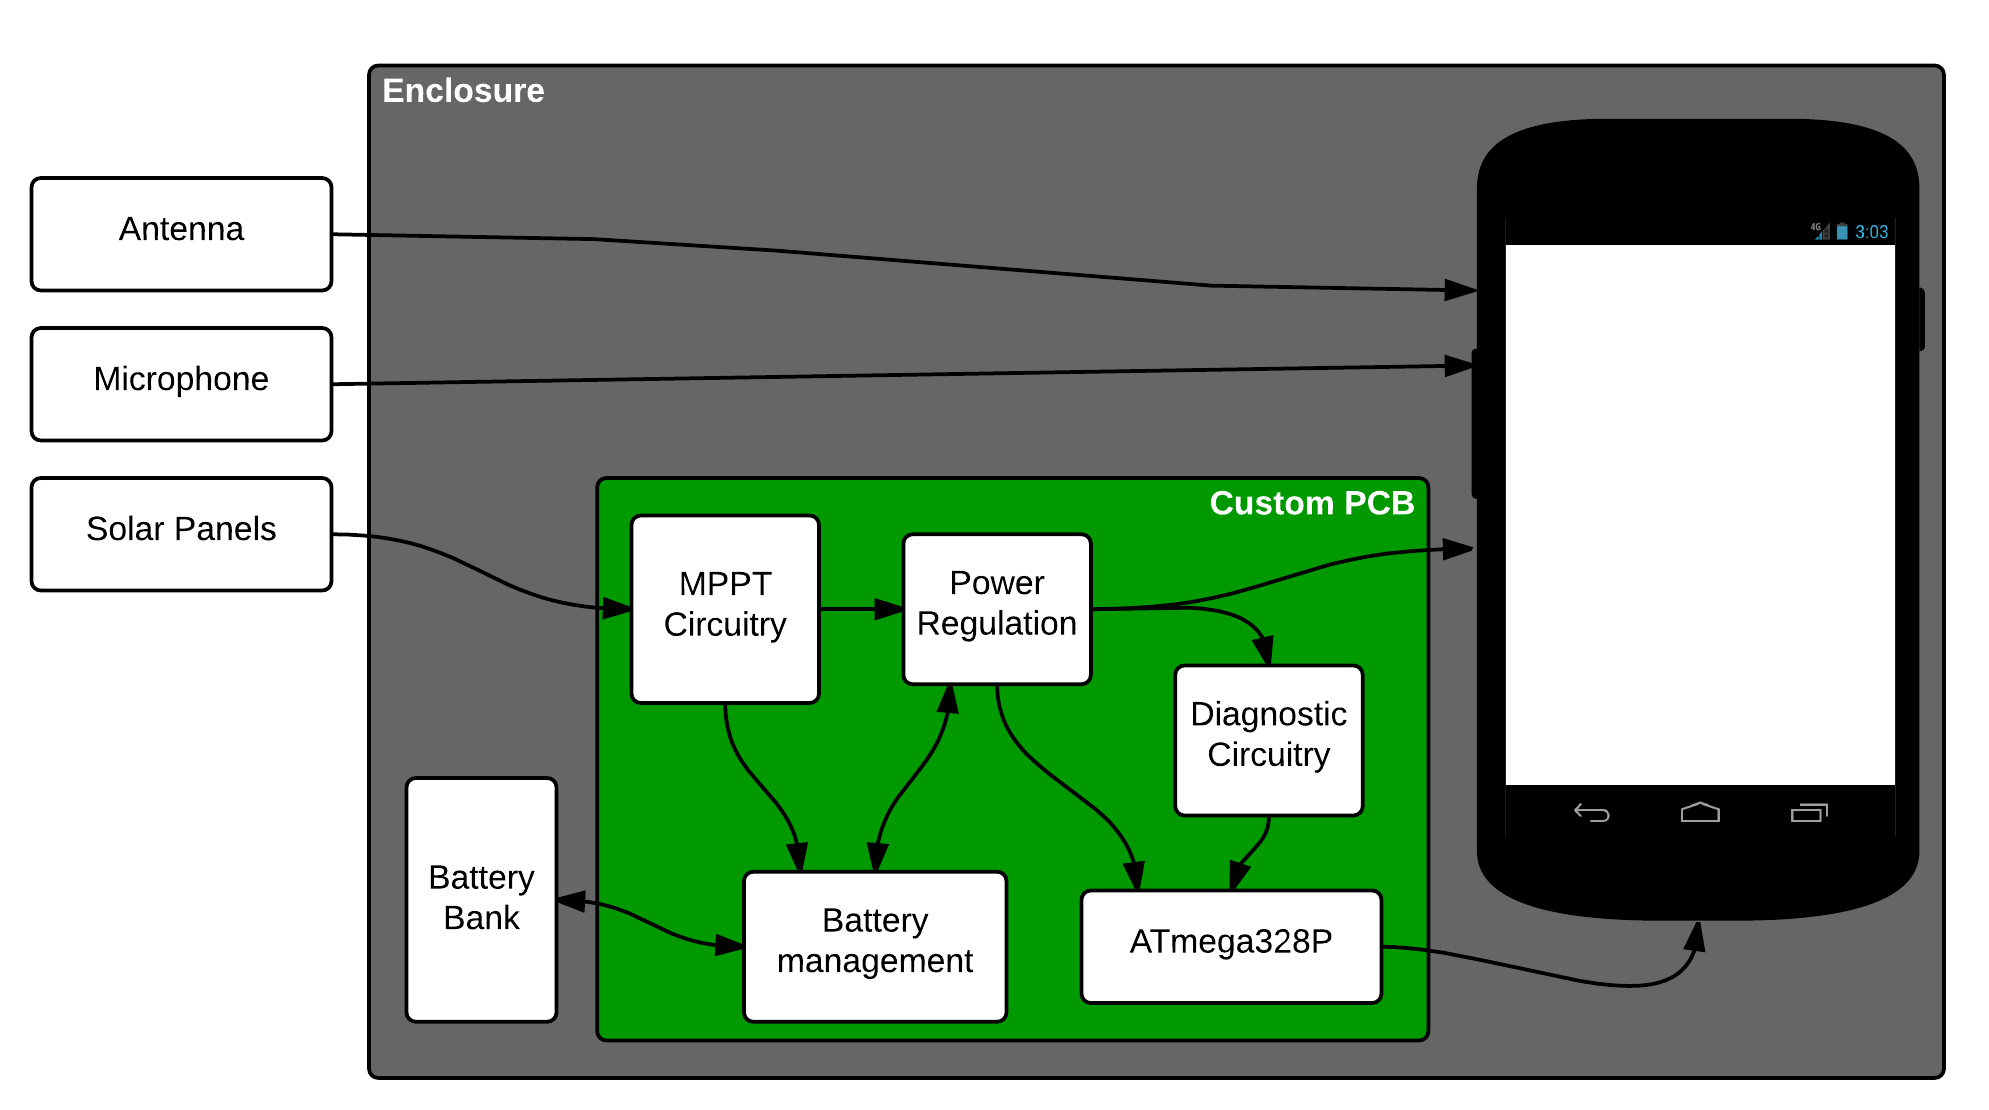
\includegraphics[width=0.8\textwidth]{Highlevel}
  \caption{High Level Functional Diagram of the Major Components}
  \label{fig:hldia}
\end{figure}

% \begin{figure}[H]
%   \centering
%   \includegraphics[width=0.8\textwidth]{DeviceDesign}
%   \caption{3D Rendering of Final Device Design: Shows the relative placement of the phone and PCB inside of the enclosure}
%   \label{fig:devdesign}
% \end{figure}

\begin{figure}[H]
	\centering
	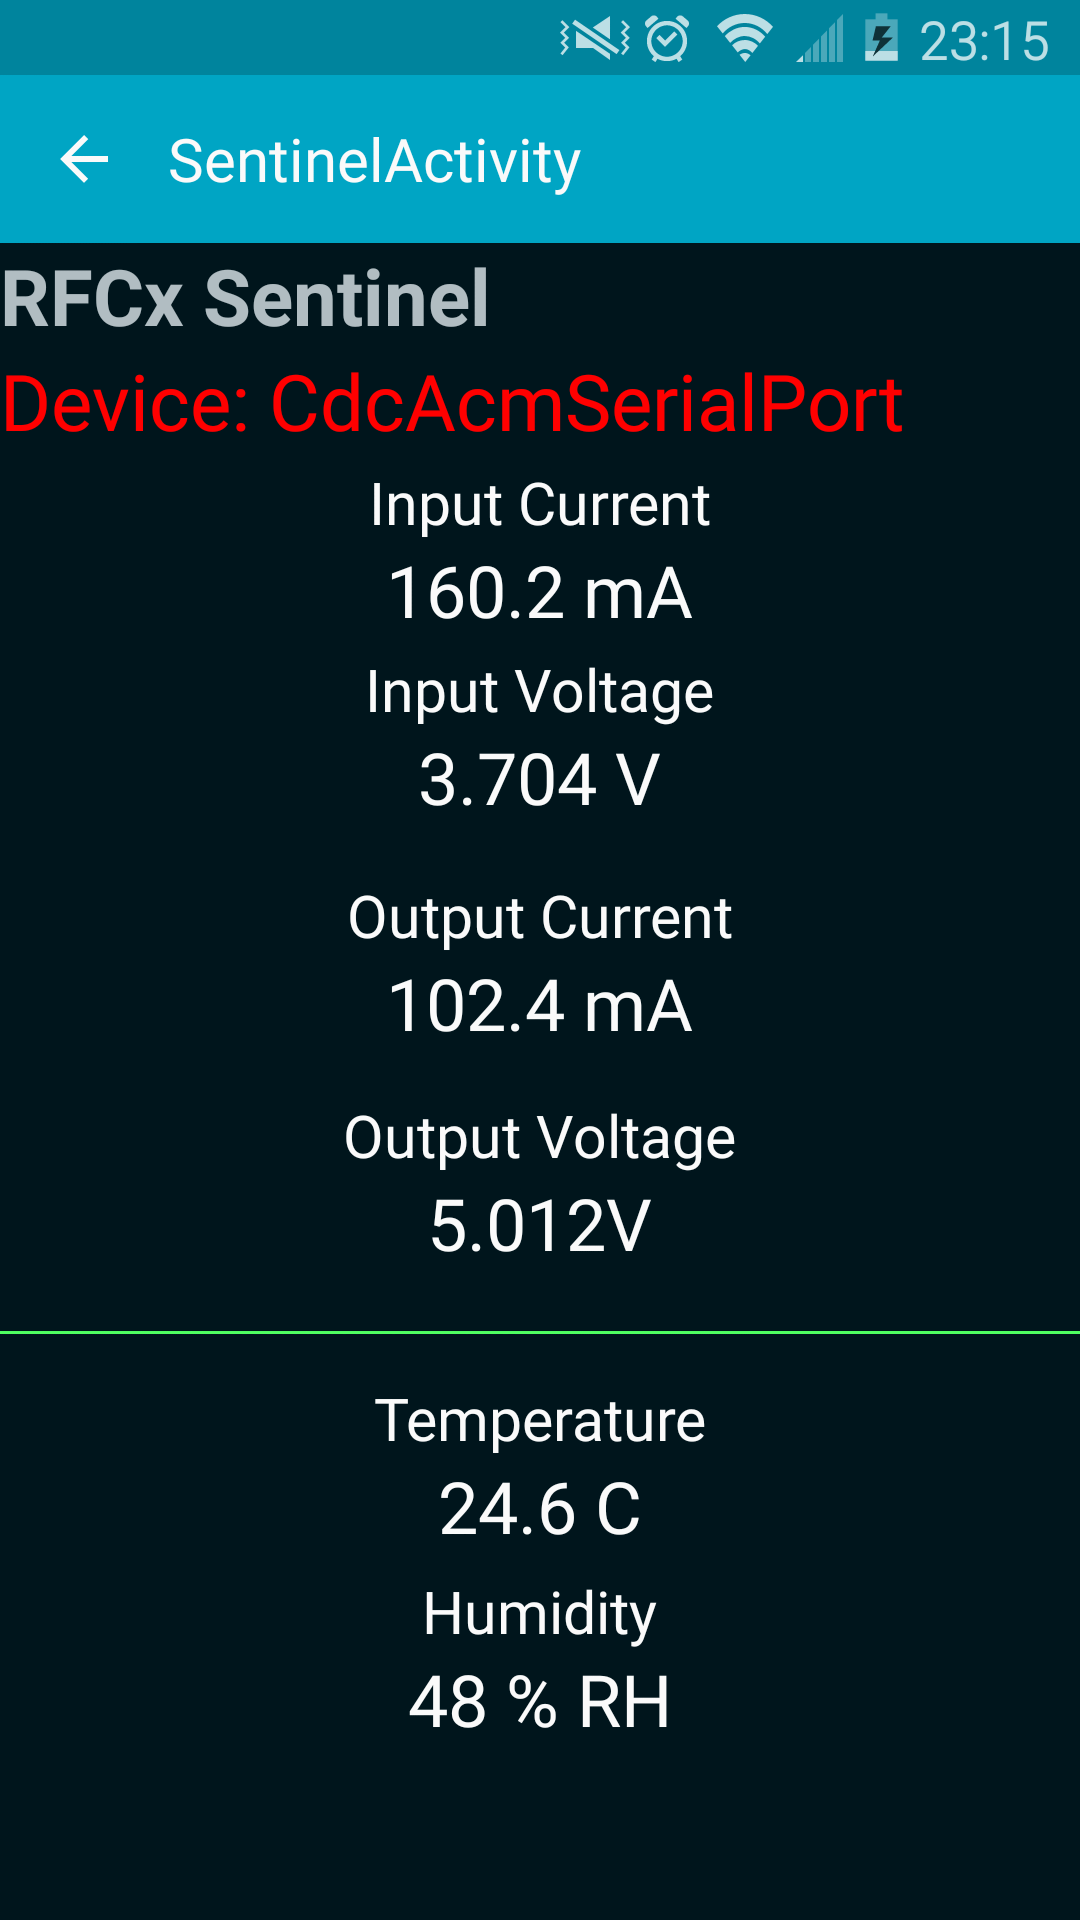
\includegraphics[width=0.4\textwidth]{RFCxSentinelScreenshot}
	\caption{Actual RFCx Sentinel App Screenshot}
	\label{fig:sentscrn}
\end{figure}
\section{Requirements and Functional Specifications}
\subsection{External Interfaces Requirements}
This section addresses the requirements of the enhanced device pertaining to its external interfaces. External interfaces are defined as components of the device interacting with something outside of the device enclosure.
\subsubsection{Hardware}
\begin{enumerate}[align=left,leftmargin=*, labelindent= 0em, label=\textbf{Requirement \thesubsubsection.\arabic*.}, itemindent=0em]

\item \label{HWa} The device shall not exceed the existing power consumption and should reduce power consumption by at least 10\%.
\item \label{HWb} The interface with the phone shall consist of a USB connection for power and data, a microphone connection via the standard audio jack, and a connection to the external antenna.
\item \label{HWc} The interface with the phone shall consist of a USB connection for power and data, a microphone connection via the standard audio jack, and a connection to the external antenna.
\item \label{HWd} Shielding techniques should be investigated to reduce the GSM audio interference noted by Topher White in the audio recordings.
\item \label{HWe} The microphone shall be interfaced via the standard audio jack on the Android phone.
\item \label{HWf} Camouflage color scheme may be used to conceal the device from loggers.  Additional camouflage features may be added so long as those features do not cover the solar panels.
\item \label{HWg} A simple assembly process shall be well documented with illustrations.

\baselinestretch
To verify \ref{HWg}. a sample group of people with varying skill levels will be asked to provide feedback on the assembly process and will be timed.

\item \label{HWh} The assembly and installation documentation may be translated into Spanish, French, and/or Portuguese.
\end{enumerate}
\subsubsection{Software}
\begin{enumerate}[align=left,leftmargin=*, labelindent= 0em, label=\textbf{Requirement \thesubsubsection.\arabic*.}, itemindent=0em]
\item \label{SWa} The algorithm used to compress the audio signal may be compared to other existing algorithms and may be changed as such depending on the outcomes of comparative testing.

\baselinestretch
To verify \ref{SWa}, audio will be recorded and compressed using multiple algorithms including the current algorithm. An infographic hosted on RFCx’s website, shown in Figure 2 illustrates the flow of data that is collected from the phone and analyzed on the server.
\end{enumerate}

\subsection{Internal Device Requirements}
This section addresses the requirements of the enhanced device pertaining to its internal interfaces and software. Internal here is defined as anything inside of the device enclosure.
\subsubsection{Hardware}
\begin{enumerate}[align=left,leftmargin=*, labelindent= 0em, label=\textbf{Requirement \thesubsubsection.\arabic*.}, itemindent=0em]
\item \label{HW1}The PCB shall consist of battery management circuitry, the power regulation circuitry, power interface to the phone, power monitoring circuitry, as well as the microphone interface.

\baselinestretch
To verify \ref{HW1}, SPICE will be used to simulate the power charging circuitry to obtain power consumption and efficiency calculations. The manufactured and assembled board will then be subjected to a load test in a lab setting.

\item \label{HW2}The device shall use the existing external microphone and antennae
\item \label{HW3}There should be a low power microcontroller included on the PCB that communicates with the Android phone. This will be used to monitor power consumption and provide external control of peripherals through the Android Debug Bridge protocol over USB. Extra general purpose IO pins of the microcontroller should be easily accessible for interfacing with future hardware.

\baselinestretch
To verify \ref{HW3}, simple packets will be sent from the microcontroller to the phone. These packets can be verified with debug tools or simple programs on the microcontroller and the phone. A debug serial port may be included as a peripheral to the microcontroller to aid in debugging. Any analog values read by the microcontroller will be verified with shop equipment.

\item \label{HW4} The monetary cost of the device, not including the solar panels, shall not exceed 25\% more than the current device cost, also not including the solar panels. The current cost of the solar panels has been quoted at \$200 and the rest of the device has been quoted at \$200. Increases in monetary cost above the current cost and below 125\% of the current cost are for enhancements in functionality (i.e. the PCB, etc.) and reductions in assembly time.

\end{enumerate}
\subsubsection{Software}
\begin{enumerate}[align=left,leftmargin=*, labelindent= 0em, label=\textbf{Requirement \thesubsubsection.\arabic*.}, itemindent=0em]
\item \label{SW1}The microcontroller software should be capable of bi-directional communication between itself and the Android phone.
\item \label{SW2}The microcontroller software should be capable of communicating power usage diagnostics to the phone over the ADB protocol.
\item \label{SW3}An Android companion application may be capable of reporting power diagnostics from the microcontroller for testing and debugging.
\item \label{SW4}There shall be a header on the PCB to program to reprogram the microcontroller.
\end{enumerate}

\section{System Architecture}
\subsection{Hardware Specifications}
\textbf{PCB}

The following is a list of the main IC’s that make up the design of this PCB
\begin{description}[font=$\bullet$\scshape\bfseries]
\item[Atmel ATMega328P]: 8-bit AVR microcontroller
\item[SPV1040 Max Point Power Tracker]: Solar power controller and lithium-ion battery charger
\item[ADS1015]: External 4-input 12-bit Analog-to-Digital Converter, I2C communication
\item[LM75BD]: Ultra Low Power Temperature Sensor,$\pm 2^{\circ}C$, I2C communication
\item[(Optional) HIH6130]: 14-bit resolution Humidity and Temperature Sensor with accuracy of $\pm4$\% Relative Humidity and $\pm 1^{\circ}C$, I2C communication
\item[FT230X]: FTDI USB-UART interface for USB serial communication
\item[bq2057CTS]: Linear Battery Charge Management IC 
\item[LM61428]: Simple Switcher Boost Controller IC
\item[SM72238]: Micropower Fixed 3.3V LDO
\item[LTC6800]: Rail-To-Rail Input and Output Instrumentation Amplifier
\item[LTC4412]: Low loss powerpath controller
\end{description}

\subsubsection{Hardware Design}

\textbf{Power Sources}

The system is powered from 8 solar cells that have been manufactured by RFCx. These solar panels have been reported to have an open circuit voltage of 1.6V and produce 0.75W each. The other power source on board is two 2-cell 4400mA/Hr lithium-ion (Li-ion) battery packs. The solar panels are going to be configured in a way that a pair may be wired in either series or parallel, which will be wired in parallel with the other three pairs. The pairs will be wired how the end user would like them and the remaining wires will be connected to a terminal block with screw/leaf spring wire termination on the PCB board, which will be powering the MPPT controllers. This is illustrated in the figure \ref{fig:mpptsol}. 

\begin{figure}[H]
	\centering
	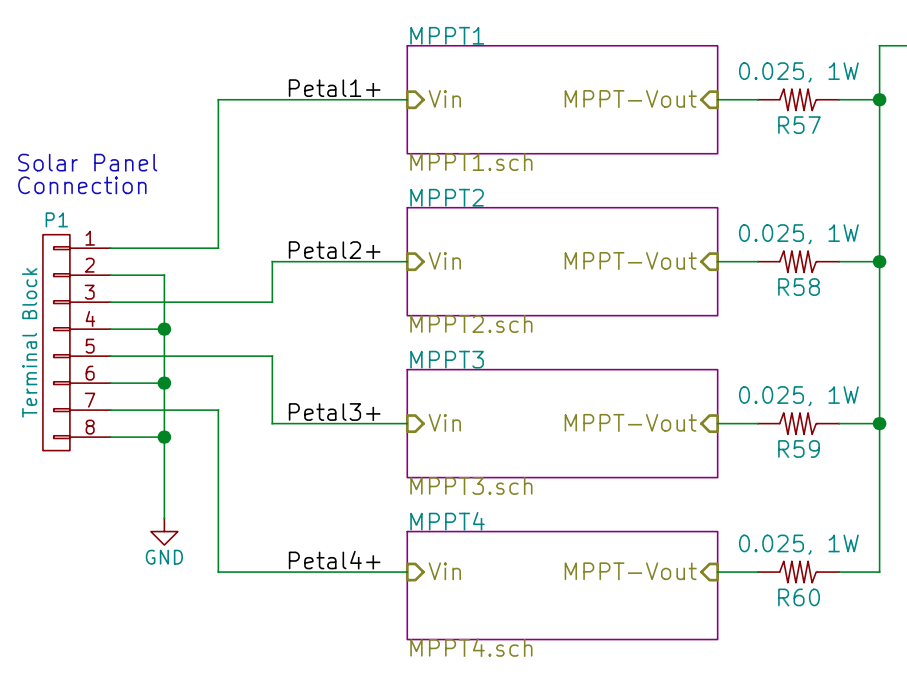
\includegraphics[width=0.4\textwidth]{MPPTblocks}
	\caption{MPPT and Solar Panel Interface}
	\label{fig:mpptsol}
\end{figure}

This configuration was chosen because the end user may decide to change the panel configuration at a later date. The optimal configuration is when each pair is in parallel. Multiple MPPT chips are required for solar panels wired together because without them the worst performing panel would dictate the output power of the whole bank of solar panels. In this configuration the output voltage will be the same and the output current will be the sum of the output current from each of the MPPT regulated series solar cells. 
\textbf{Solar Charging}

Instead of the currently used solar power regulator (MCP73871 on an Adafruit board), the SPV1040 Max Point Power Tracker(MPPT) will be used. The MCP73871 is a linear battery charger and management IC that is meant to charge a single cell Li-ion battery, however there are 4 in this system. The MCP73871 is also only available in a QFN package, which will make assembly harder for the end user. An MPPT increases efficiency by adjusting the current and voltage of the output to achieve the maximum power. The MPPT IC will regulate the solar cell voltage up to 5.2V. From the MPPT IC, the battery management circuitry, the 3.3V line, and the 5V line is powered.The SPV1040 was chosen for two reasons: RFCx currently has a multitude of them in stock, and suggested that we use them, and they require less control and I/O than the Solar Magic SM72442, a similar MPPT chip that was also considered, but which requires more power and more control from the MCU via an I2C interface.

\textbf{Battery Management}
The BQ2057CTS is a charge management IC designed for single and dual cell Li-ion battery packs. Battery management is very important because if a battery is damaged by over or under charging and it goes unnoticed it could sink current from the other batteries or discharge into the other batteries causing more damage and possibly catch fire. This system is meant to be mounted in remote and hot climates, so safe battery management is a concern. One of these IC’s are used for each of the two 2-cell battery packs. This battery management IC combines current and voltage regulation, charge status indication, and charge rate auto compensation. It also comes in an easy to use surface mount package. The charge rate auto compensation feature allows the batteries to charge faster by compensating for internal impedance of the battery pack. This IC was chosen for its charging features, its ability to handle two cells, its indication capabilities, as well as the package it comes in. The following figure shows the battery management circuitry for one of the 2-cell battery packs.

\begin{figure}[H]
	\centering
	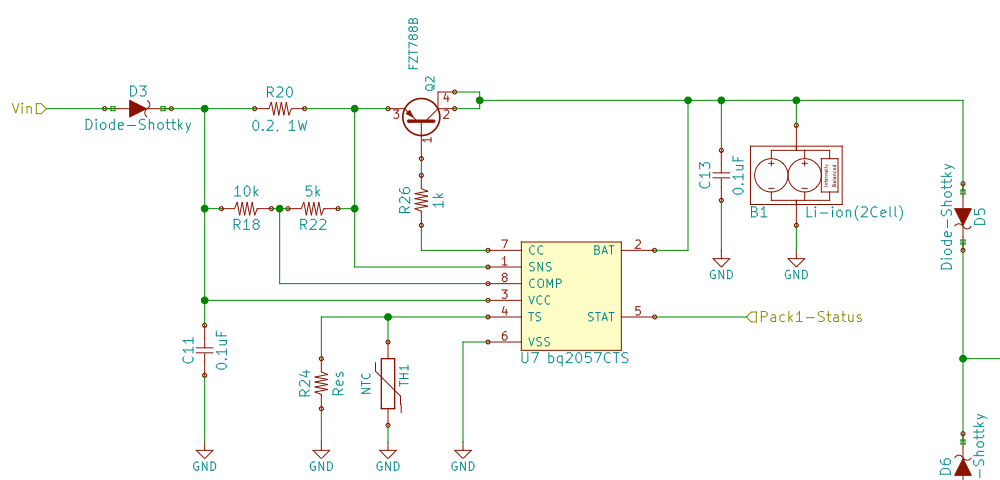
\includegraphics[width=0.4\textwidth]{BatteryManage}
	\caption{Battery Management Circuitry}
	\label{fig:batman}
\end{figure}

The calculations for the component selection for the battery management circuitry is included in the Appendix.

\textbf{Voltage Regulation}

A diode-ORed power path management circuit was used to switch the power source that feeds the 3.3V and 5V regulation circuitry. This circuit is shown below. 
\begin{figure}[H]
	\centering
	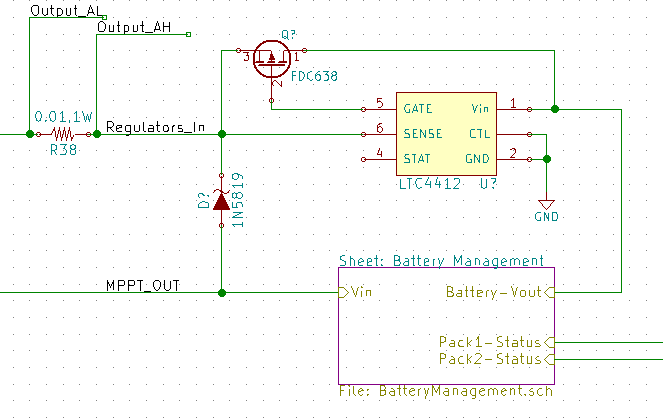
\includegraphics[width=0.4\textwidth]{DiodeOR}
	\caption{Diode Ored Circuit}
	\label{fig:dored}
\end{figure}
The reason this circuit was chosen is because power path switching happens in under 100us and there is no dip in the output voltage. This dip was observed in a simulation of a different power path switching topology that involved only the FET and the diode. The two circuits were simulated with LTSpice and can be seen in figure x. The same diode and transistor were used in each simulation. A load of 550mA was used because this is more than the calculated worst case current draw from the circuit. 

\begin{figure}[H]
	\centering
	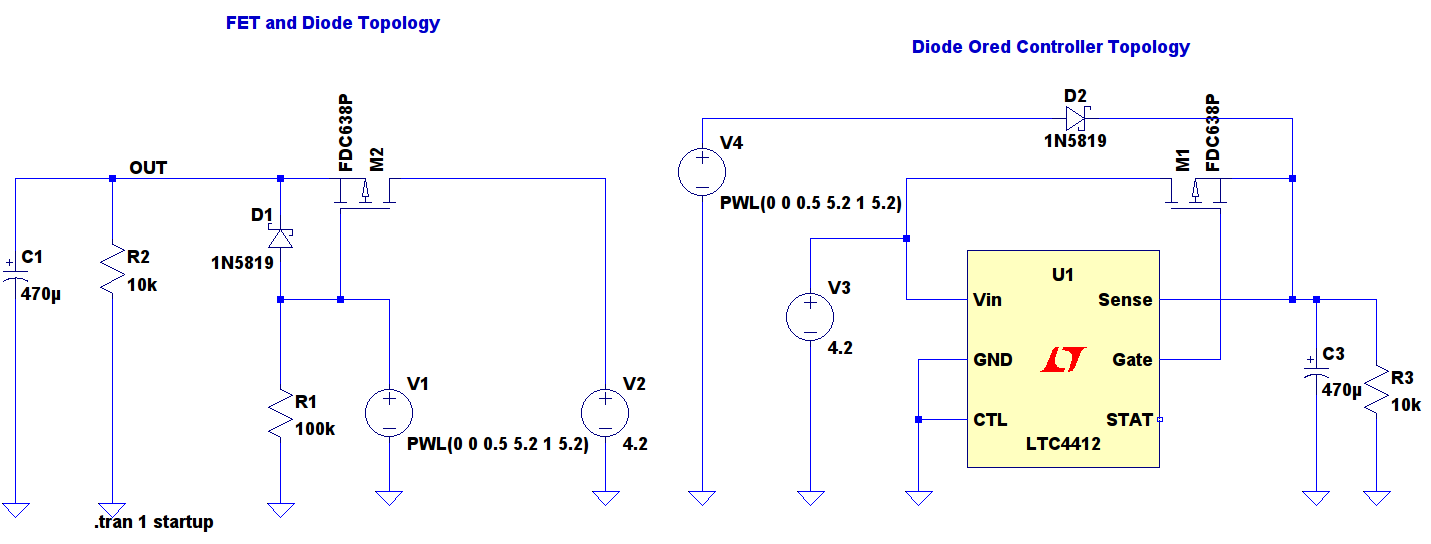
\includegraphics[width=0.4\textwidth]{DiodeORSIM}
	\caption{Simulation of Diode Ored Circuit}
	\label{fig:doredsim}
\end{figure}

The transient simulation results of the diode and transistor topology can be seen in the following figure.

\begin{figure}[H]
	\centering
	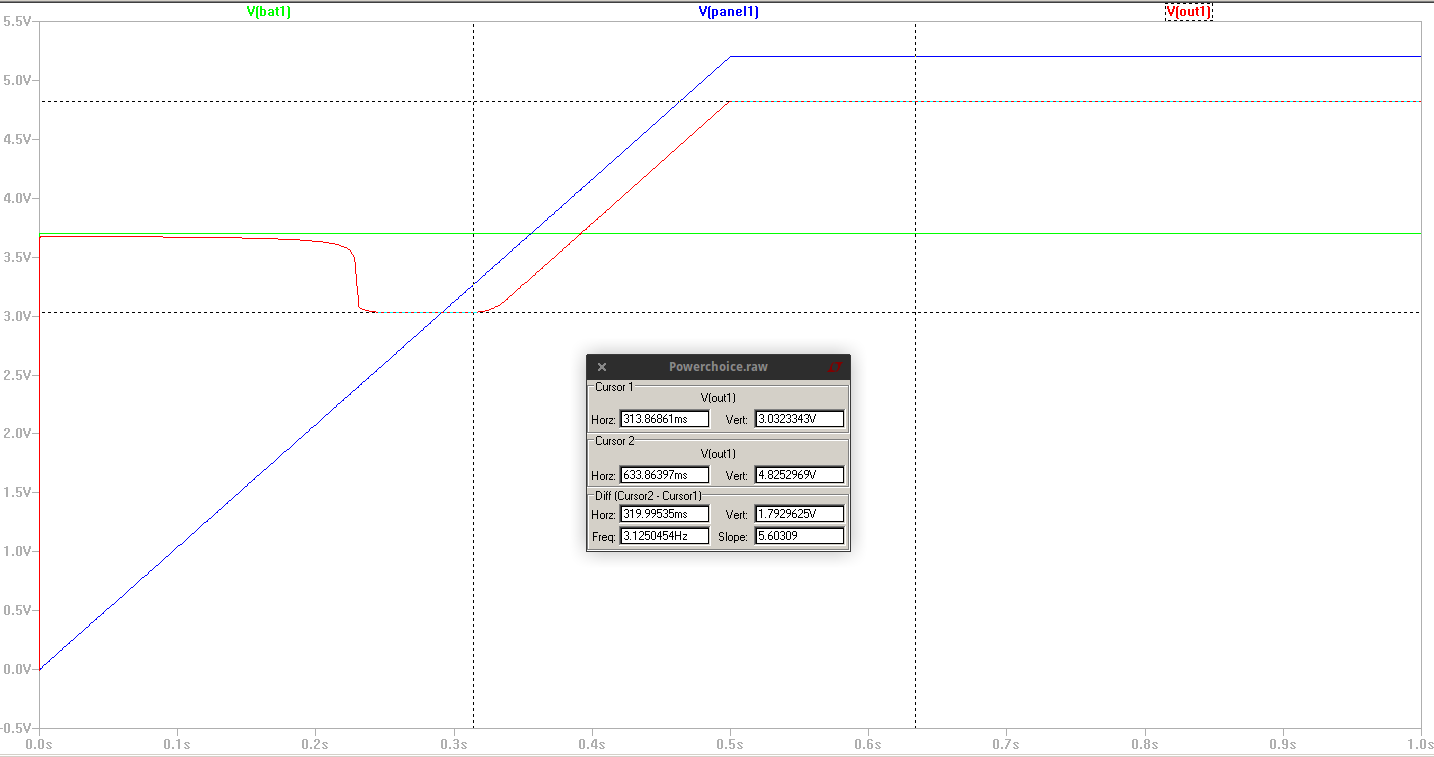
\includegraphics[width=0.4\textwidth]{DiodeORres1}
	\caption{Simulation Result of Old Diode Ored Circuit}
	\label{fig:doredsimres1}
\end{figure}
It can be seen that as the panel voltage is rising, there is a considerable dip to around 3.0V. If this occured, the 3.3V linear drop out regulator would not be able to regulate properly and the 3.3V line would be deactivated. The diode-ored controller topology simulation result can be seen in the following figure.
\begin{figure}[H]
	\centering
	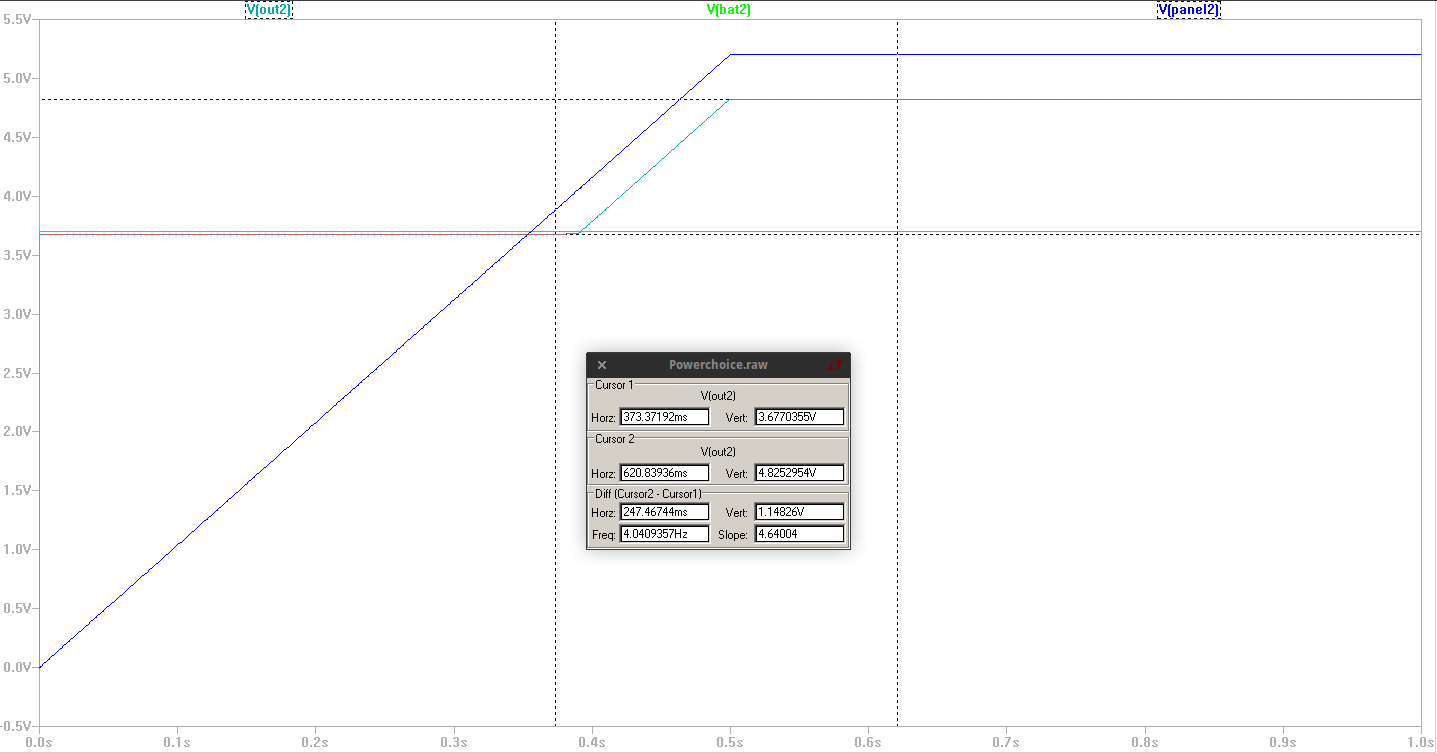
\includegraphics[width=0.4\textwidth]{DiodeORres2}
	\caption{Simulation Result of Current Diode Ored Circuit}
	\label{fig:doredsimres2}
\end{figure}

Here it can be seen that there is a very small drop in voltage when powered only from battery and a reasonable drop when powered from the solar panel. This is the desired behavior. The supporting components were chosen because they were suggested in the LTC4412 data sheet and they were in reasonable packages for the end user to assemble with.

The LM61428 is a step-up voltage regulator that is configured to boost the input voltage to 5V and an output current of up to 1A. The reason for this voltage is to charge the cell phone battery.
The calculations for the surrounding components can be seen in the Appendix. The layout of the 5V boost regulator can be seen in the following figure.
\begin{figure}[H]
	\centering
	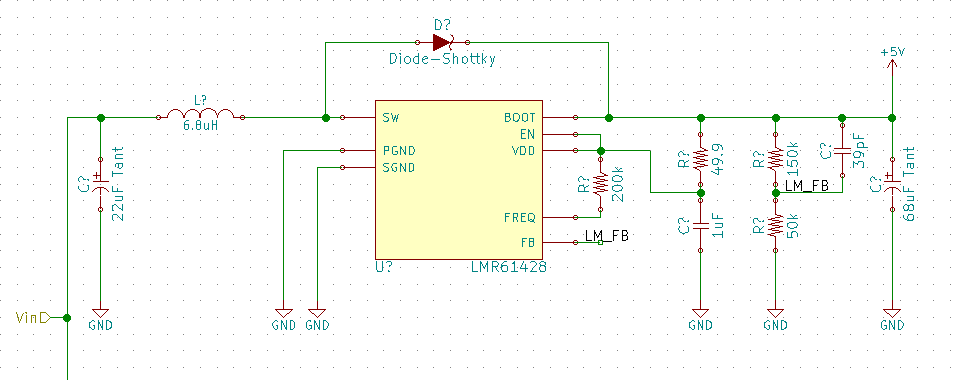
\includegraphics[width=0.4\textwidth]{PS5V}
	\caption{5V Voltage Regulation}
	\label{fig:ps5}
\end{figure}
A Texas Instruments SM72238 Micropower fixed 3.3V LDO is used to regulate the 3.3V line. This was chosen over a switching regulator because the minimum voltage of 3.7 and the output voltage of 3.3V were too close together, causing the duty cycle calculations to come out to negative or not meet certain regulator’s requirements. The SM72238 has very low dropout, which is in range for the need of this application. The only external components required by the LDO are two low ESR 1uF capacitors on the input and output. 

\textbf{Input and Output Current and Voltage Sensing}
The ADS1015 is a 12-bit ADC that can communicate over I2C with the microcontroller. An external ADC is used here because fewer I/O lines are used on the microcontoller and this has a higher resolution. 

The LTC6800 instrumentation amplifier is used to sense the voltage across a known sense resistor. This is so that the ADC can read the output and the current that is being drawn by the circuit can be calculated by the microcontroller. The input current sense circuit is configured to have a gain of around 80.5. The sense resistor has been selected to be 0.01 Ohms. With this configuration the ADC will be able to sense the current with a resolution of 1mA/bit. The calculations for this section can be seen in the Appendix. The configuration of the current sense amplifier can be seen in the following figure.
\begin{figure}[H]
	\centering
	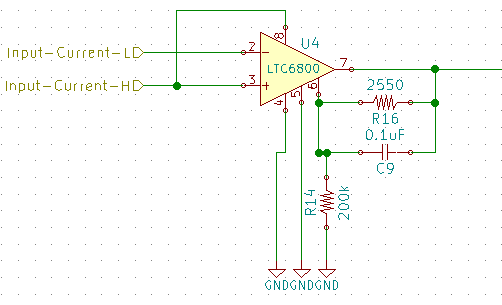
\includegraphics[width=0.4\textwidth]{AtoV}
	\caption{Current Sense Amplifier}
	\label{fig:AV}
\end{figure}

The LTC6800 is used to sense the input and the output current. The input and output voltage are sensed with simple resistor dividers that are fed to the ADC. 

\textbf{Microcontroller}


The purpose of having a microcontroller on board was to be able to relay diagnostic information of the environment to the phone so that it may take the information into consideration with its own calculations. The common Atmel ATmega328P and an FTDI IC were chosen to be the interface between the phone and the on board diagnostic circuitry. 

Three other microcontrollers were considered. Two ARM M0+ low power micro controllers were considered. The Atmel ATSAM ARM M0+ was not chosen because it drew more current than the 328P and was decided to be over kill for this application. Some nice features were that it had a built in USB module and required no external tools to program it. The Freescale KL25Z was also decided to be overkill for this application and was not chosen because the programming interface of the end user would have been difficult as it required a JTAG programmer. The other microcontroller was a Texas Instruments 16-bit RISC MSP430. This microcontroller was the most expensive, drew the highest current in active and sleep modes, and requires an external tool to program. The ATmega328P does require an external tool to program but it does have low power sleep modes, it is cheap, its is simple, and it is well documented not only by Atmel but by a very large community. It is felt that this would benefit the end user the most in the future. 

\textbf{Temperature and Humidity}

A temperature sensor (LM75BD) and a humidity/temperature sensor(HIH6130) are going to be designed onto this board. It is not intended that they both be populated at the same time but it does give the end user an option in case humidity is not a concern or the HIH6130 is too expensive. Both ICs are low power and communicate with the microcontroller over I2C. The schematic connections of the two ICs is shown in the following figure.

\begin{figure}[H]
	\centering
	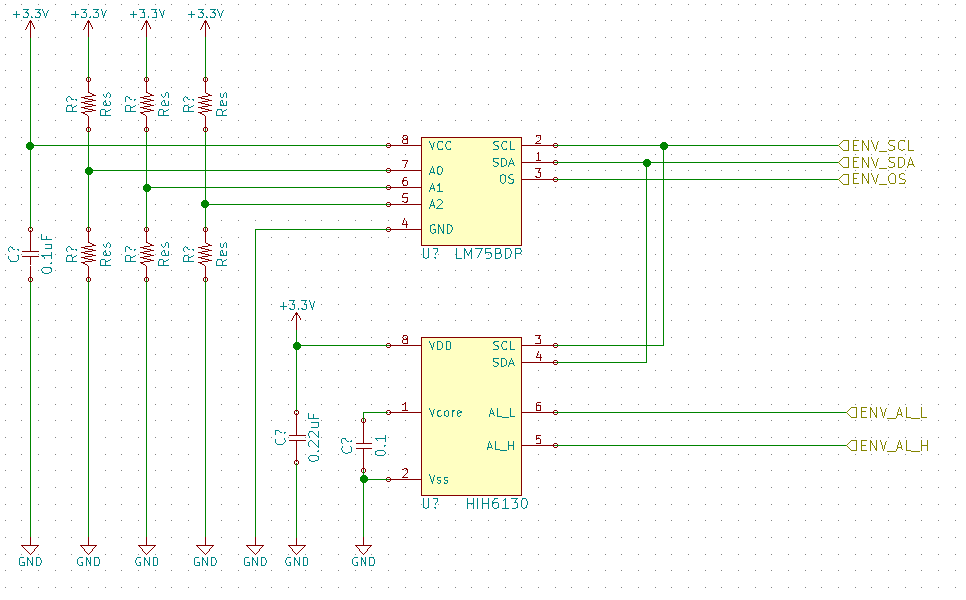
\includegraphics[width=0.4\textwidth]{temphumid}
	\caption{Temperature and Humidity Sensors}
	\label{fig:tandh}
\end{figure}

\textbf{Connectors}

The USB connection consists of a standard USB Micro A connector, soldered directly onto the board and is secured to the board as a strain-relief mechanism. A standard 3.5mm audio cable is used to connect the microphone. A standard GSM antenna adapter is used to interface with the phone’s onboard GSM module.

\textbf{GSM Interface}

The use of X2Y TDMA filtering capacitors will be tested to reduce the noise produced by the stopping and starting of GSM packets, which is in the audible range at ~217Hz. A pass-through 3.5mm microphone interface will be included to test the X2Y capacitors. In addition, a large heatsink will be attached to a large ground plane on one side of the board, and the phone will be attached to the same ground plane, which should help with some shielding.

\textbf{PCB Size}

Two size options were proposed for the PCB, including having only enough space for the components and having a long open space on the PCB for attaching the phone. Having a long PBC with space for the phone was chosen to simplify the assembly process for the device. The length of the open space is long enough to accommodate large phones, and variable length mounting holes in the PCB allow for any size phone to be securely mounted to the PCB using snap-fit mounting screws. A micro-USB cable is used to interface the phone to the rest of the board. Using a cable instead of a connector allows the use of any size phone in the device. Having the PCB only large enough to fit the electrical components on it requires a separate mounting mechanism for the phone, which complicates the assembly of the device.

\textbf{Heat Dissipation}
Multiple alternatives were explored for dissipating heat built up in the enclosure, including drilling holes into the enclosure, putting fans in the enclosure to control airflow in and out of the enclosure, and using a heat sink. Using a heat sink was chosen as the best design alternative for heat dissipation. Drilling holes in the enclosure can allow water, insects and dust to enter the enclosure. A wire mesh over the holes could be used to keep insects out of the enclosure, but water and dust could still get into the enclosure and damage the electronics. Running fans in the device creates a sound in a similar frequency range to the chainsaw noise the device is trying to detect. This can cause false detection of a chainsaw by the RFCx server. A heat sink also requires a hole to be drilled into the enclosure for the heat sink to reach outside of the enclosure. This opening is sealed with caulk or by other methods to prevent water, insects and dust from entering the enclosure. The battery cover on the phone is removed and thermal paste is used between the phone battery and the PBC, and between the PCB and the heat sink. This allows heat to dissipate out of the enclosure and help keep the phone attached to the PCB and the PCB attached to the heat sink. Vias in the PCB help heat to transfer more readily through the board instead of trying to transfer the heat through the fiberglass the board is made of.

\subsubsection{Hardware Implementation}
\textbf{Heat Sink}
A heat sink, as described in Section 3.1.1 is shown in Figure 1.4.  The current design calls for a rectangular opening to be cut into the front face of the enclosure so that the heat sink may pass through.  The shape of the heat sink will be optimized for reduced interior air temperature through heat transfer calculations.

\subsection{Software Specifications}
The software used in the design will consists of C and C++ code running on the ATMega328P microcontroller, as well as a companion app (RFCx Sentinel) written in Java, running on the Android phone.
\begin{figure}[H]
	\centering
	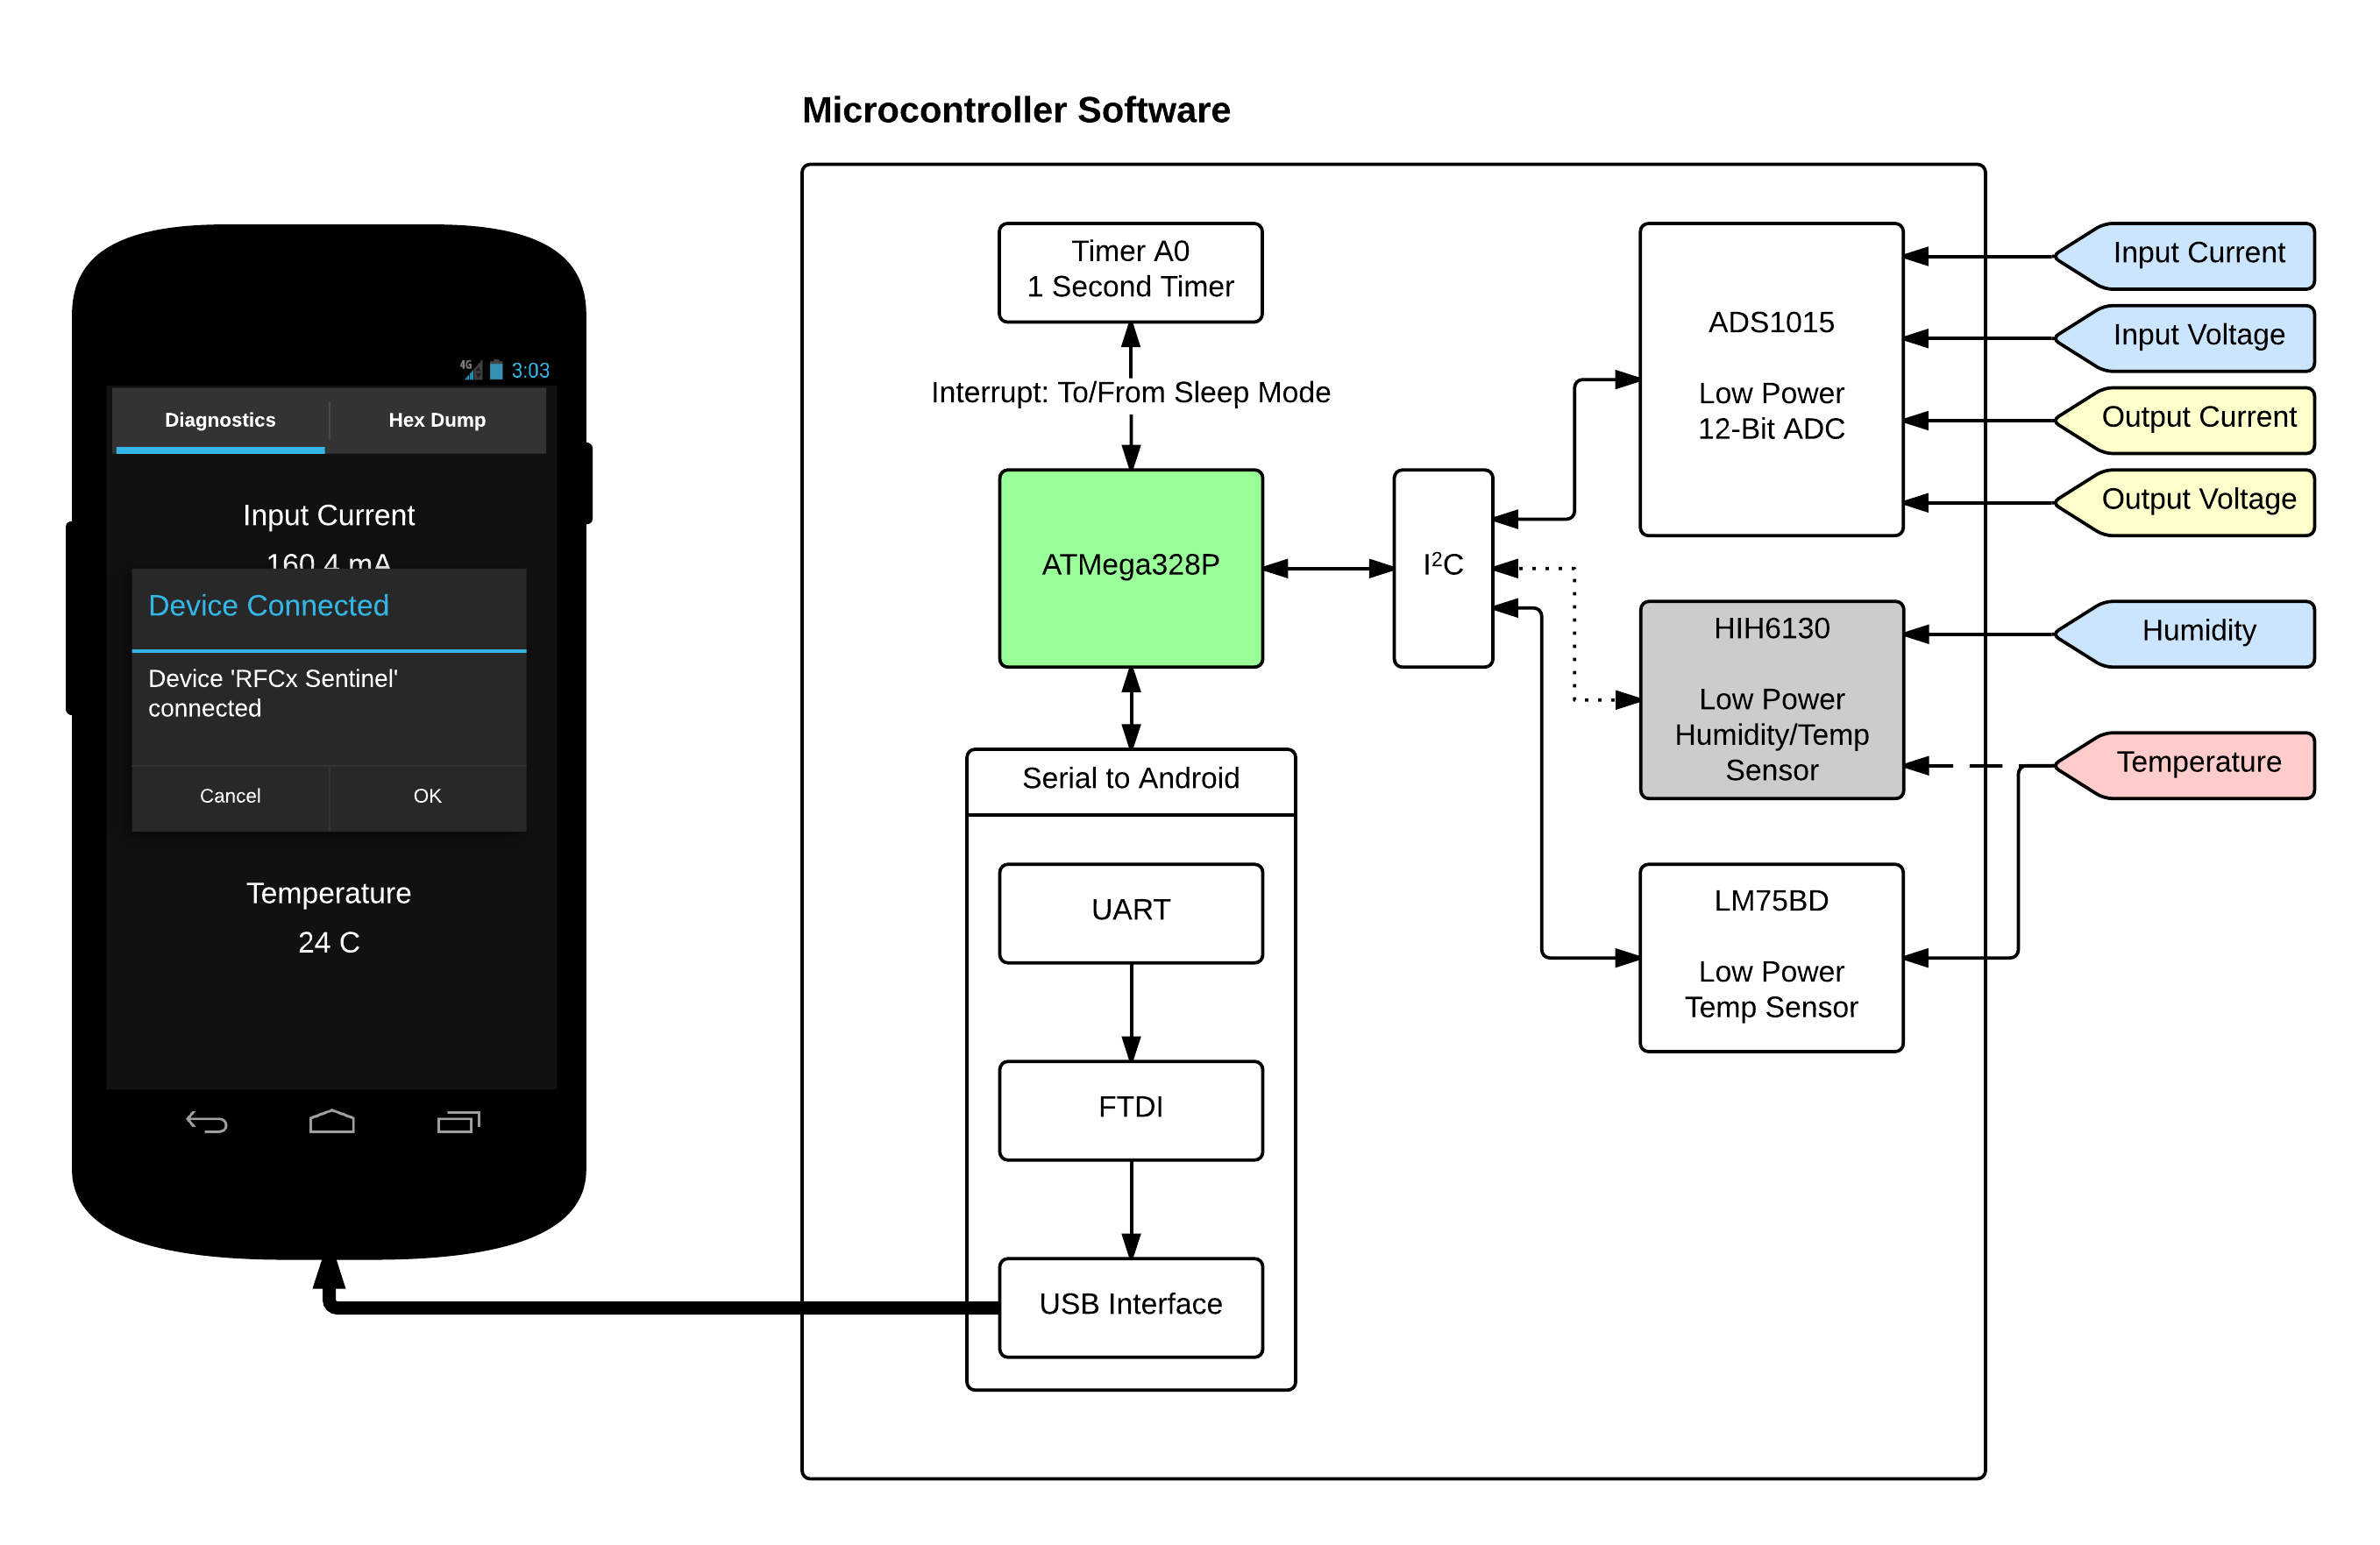
\includegraphics[width=0.4\textwidth]{SoftwareUMLV2}
	\caption{Software UML Diagram}
	\label{fig:swuml}
\end{figure}

\subsubsection{Software Design}
The microcontroller software gathers data from a humidity/temperature sensor, and input/output current and voltage. This data is sent via the ATMega328P serial port to the Android phone via the FTDI chip on the PCB and the usb-serial-for-android libraries on the phone.
Listing \ref{lst:snip} describes the basic functionality of the microcontroller software.

\begin{lstlisting}[language=C,label=lst:snip,caption=MCU Flow Code Snippet]
void wakeFromSleep() {
    //Get sensor measurements
    GetDiagnostics(&Diagnostics);
    //Send sensor measurements to phone
    SendDiagnostics(Diagnostics);
    //Go to sleep
    enterSleep();
}
\end{lstlisting}

\subsubsection{Software Implementation}
An ATMega328P microcontroller is be used to take measurements from the sensors. The temperature (and possibly humidity) measurements are sent digitally via I2C to the microcontroller. On the same I2C bus is the ADS1015, which has four single-ended analog inputs for reading the input current, input voltage, output current, and output voltage. This data is be sent to the phone using the standard AVR UART serial library.

The data, once sent to the phone, is be monitored by the RFCx Sentinel app. This app is written in Java in Android Studio, and uses the open-source usb-serial-for-android library. The app opens a connection upon discovering a compatible device (FTDI is compatible), and allows the user to view a streamlined interface with relevant data, as well as a tab for the raw hex dump of incoming serial data. The data may or may not be transmitted along with audio data to the RFCx server for real-time monitoring.


\section{Verification}
\subsection{Hardware Verification}
To verify the power consumption of the devices in Requirement 2.1.1.1. the voltage applied and current drawn by the both the enhanced device and the current device will be measured over the course of 1 hour during a realistic usage scenario. The average power will be verified to not exceed 90\% of the existing device’s usage.

To verify Requirement 2.1.1.5. a visual inspection by volunteers will qualify camouflage schemes. A successful inspection will be one in which more than 80\% of the volunteers are unable to find the device within a 2 minute inspection window.

To verify Requirement 2.1.1.6. a sample group of people with varying skill levels will be asked to provide feedback on the assembly process.

\subsection{Software Verification}
To verify Requirement 2.1.2.1., audio will be recorded and compressed using multiple algorithms including the current algorithm. An infographic hosted on RFCx’s website, shown in Figure 2 illustrates the flow of data that is collected from the phone and analyzed on the server.

To verify Requirement 2.2.1.3., simple packets will be sent from the microcontroller to the phone. These packets can be verified with debug tools or simple programs on the microcontroller and the phone. A debug serial port may be included as a peripheral to the microcontroller to aid in debugging. Any analog values read by the microcontroller will be verified with shop equipment.

\section{Validation}
Requirements 2.2.1.2, 2.1.1.2, and 2.1.1.4 can be validated by inspecting the components on the PCB to ensure all required components are present on the board. Requirements 2.1.1.6 and 2.1.1.7 can be validated by handing the assembly instructions out to a sample group of people with varying skill levels and receiving feedback on the set of instructions from them. People with the ability to read other languages can be used if the documents have been translated from English into other languages.

Requirement 2.2.1.4 can be validated by inspecting the total cost printed on the BOM for the enhanced device.

Requirements 2.2.1.1, 2.1.1.1, and 2.2.1.3 can be validated by current and voltage measurements taken in the lab using a DMM. The power calculations made based on those measurements can be compared to similar calculations based on measurements taken from the current device. SPICE simulation data and values displayed on the RFCx Sentinel app will be compared to the actual power consumption of the new device.

Requirement 2.2.2.1, 2.2.2.2, 2.2.2.3, and 2.2.1.3 can be validated by comparing the values reported in the RFCx Sentinel app to the calculated power consumption of the enhanced device.

Requirement 2.1.1.3 can be validated by changing the scale factor in the microcontroller program, reprogramming the microcontroller from the PCB header and comparing the values displayed on the RFCx Sentinel app to the previous displayed values. The new values displayed on the RFCx Sentinel app should reflect the change to the scale factor in the microcontroller program.

Requirement 2.1.1.3, 2.2.2.3, and 2.1.2.1 can be validated during a field test. The enhance device can be mounted at eye level in a tree and turned on to allow the device to start sending audio data to the RFCx server. Requirement 2.1.1.5 can be validated by having a volunteer outside of the project search for the device in a wooded area without knowing what it looks like to see if it sticks out. A chainsaw can be turned on 0.25 miles from the device to trigger an alert and validate that the enhanced device can communicate with the RFCx server. The size of the audio recording sent to the RFCx server after employing the audio compression algorithm can be compared to the size of audio data sent to the RFCx server by the current device to determine the audio compression ratio of this algorithm. Both audio recordings can be played back to determine the level of audio interference created by GSM transmission.

\section{Project Budget and Schedule}
\subsection{Budget}
This project will require minor funding for manufacturing and populating the PCB, and the materials to construct a new enclosure, as well as general testing and component costs. As RFCx is a non-profit organization working solely on grant money, this budget is not expected to be covered by them.
\begin{itemize}
\item \$400 = 4 x \$100 for PCB manufacturing
\item \$320 = 4 x \$80 for PCB components
\item \$200 = 1 x \$200 for general needs
\item Estimated Total: \$920
\end{itemize}

\section{Schedule}
The schedule in Figure 6.2 is the proposed schedule for all phases of the project. This will be used as a general timeline for guidance throughout the project.


\newpage
\section*{Appendix A: Electrical Schematics}

\newpage
\section*{Appendix B: Bill Of Materials}

\newpage
\section*{Appendix C: Mechanical Drawings}

\newpage
\section*{Appendix D: Calculations}

\newpage
\section*{Appendix E: Data Sheet Snippets}
\begin{figure}[H]
	\centering
	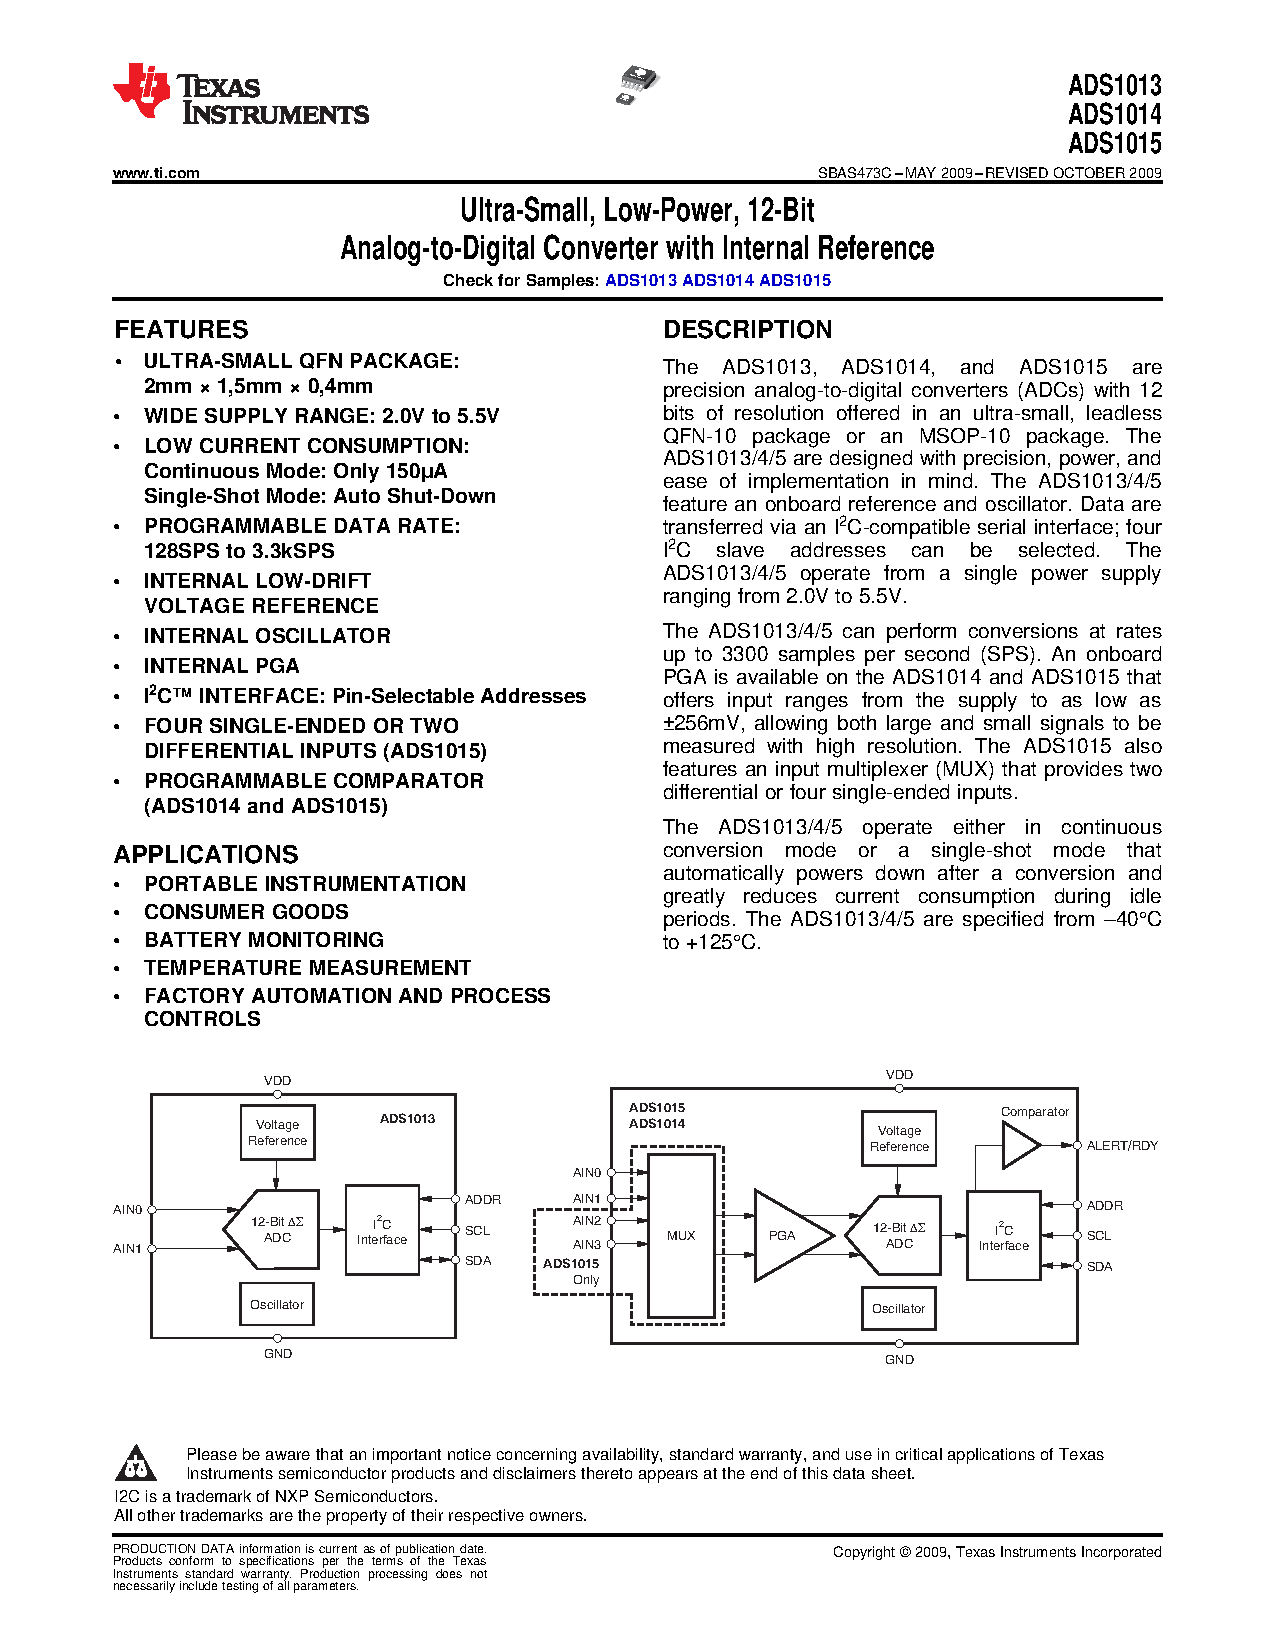
\includegraphics[page=1,width=0.9\textwidth]{combined.pdf}
	\caption{1st Page of ADS1013 Datasheet}
	\label{fig:adsdat}
\end{figure}
\newpage
\begin{figure}[H]
	\centering
	\includegraphics[page=2,width=0.9\textwidth]{combined.pdf}
	\caption{1st Page of ATmega328P Datasheet}
	\label{fig:atmeldat}
\end{figure}

\newpage
\section*{Appendix F: Source Code}
\end{document}

% ======== For Reference =============
% H parameter for the figure environment
% keeps it from floating
\begin{figure}[H]
	\centering
	\includegraphics[width=0.8\textwidth]{FIG2_1b}
	\caption{Convolution of Identical Unit Step Sequences}
	\label{fig:21b}
\end{figure}
% To turn off caption numbering place this:
%\captionsetup[figure]{labelformat=empty}
% Before the figure, To turn back on:
%captionsetup[figure]{labelformat=default}
\begin{equation}
	\begin{array}{rcl}

	y[n] &=& 0.5x[n]+x[n-1]+2x[n-2]\\
	y[n] &=& 0.8y[n-1]+2x[n]\\
	y[n]-0.8y[n-1] &=& 2x[n-1]
	\end{array}
\end{equation}

\begin{subequations}
	\begin{align}
		h[n] &= 2\delta[n+1]-2\delta[n-1]\\
		x[n] &= \delta[n] + \delta[n-2]
	\end{align}
\end{subequations}

% Resize used to make table width of text, may be omitted
\begin{table}[h]
\resizebox{\textwidth}{!}{
\centering
\begin{tabular}{|c|c|c|c|}
\hline
Case & $Z_c$          & $l$           & $c$       \\ \hline
1    & $110.9 \Omega$ & 0.593 $\mu H$ & 0.048 nF  \\ \hline
2    & $171.3 \Omega$ & 0.803 $\mu H$  & 27.408 pF \\ \hline
3    & $327.3 \Omega$ & 1.102 $\mu H$  & 10.294 pF \\ \hline
\end{tabular}}
\caption{Calculated Parameters}
\label{tbl:calcd}
\end{table}

% Code Snippet:
\begin{lstlisting}[language=C,label=lala,caption=this thing]
  code snippet
\end{lstlisting}

% bulleted list
\begin{itemize}
\item this is an item
\end{itemize}

\renewcommand*\contentsname{ }
\tableofcontents
\listoffigures

